\section{Motivation}

Satellite data transmissions have become a key part of critical infrastructure for private, national, and scientific use.
Although new satellites are being launched at a high rate, even decades-old satellites are seeing novel use cases including advanced forest fire detection~\cite{nasaFirms}, analysis of activities in conflict areas~\cite{separatistLuminosity}, emergency communications~\cite{apple_emergency_sos}, and internet service~\textbf{TODO: find citation for e.g. Iridium}.
These systems were built when robust cryptography was uncommon due to less powerful onboard computers.
% Should I note that these systems also include satellites with leaked keys etc.?

It is now well accepted that legacy communications systems without resilient authentication are not robust against modern adversaries.
However, this was often not a practical concern at the time since attacks at the physical layer would have required a costly and highly specialized setup.
Additionally, long mission lifespans have lead to a proliferation of satellites that were considered secure at launch, but have since had their master keys leaked or reverse engineered~\cite{lrit-key-dec,xrit-rx}.

Recent work has considered the impact of eavesdropping and signal injection against specific systems such as GPS.
For example, Pavur et. al. have demonstrated that high quantities of satellite internet traffic is conducted in plain HTTP through unencrypted satellite data links.  \cite{pavur2020tale}
However, no current work seeks to understand the effects of a modern adversary spoofing non-GPS satellites through signal injection.

Recent decades have seen a significant rise in the off-the-shelf availability of software-defined radio hardware, which is capable of emitting arbitrary signals at a wide range of frequencies.
This lowers the barrier to entry for signal injection and denial of service across many wireless systems, including WiFi, wireless sensors, mobile internet~\cite{yang2019hiding,erni2021adaptover}, GNSS~\cite{tippenhauer2011requirements}, and even avionic systems~\cite{sathayeWireless2019}.

However, the practicality of performing these attacks on satellites is currently unknown.
The physical layer presents unique challenges, with satellite radio frequency bands usually outside of the operating range of SDRs.
Open questions also surround the hardware setup, given that receiving stations are designed to expect a polarised signal within a single beam.
The design of the protocol may also have an impact; features such as timestamps and checksums can be used to detect simple overshadowing attacks.

\begin{figure}
    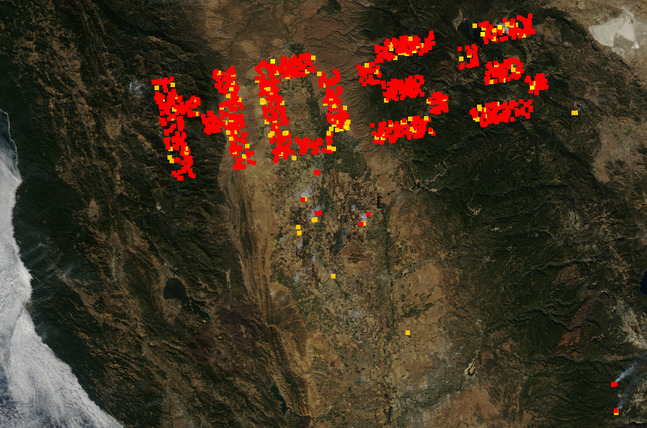
\includegraphics[width=\columnwidth]{diagrams/injection/pixels_800_140.jpg}
    \caption{An injected signal from the attacker manipulates the infrared channels of satellite imagery to create ficticious fires in the resulting dataset.}
    \label{fig:location-injection}
\end{figure}

The security community is becoming increasingly aware that radio overshadowing in a satellite context has the potential to affect critical services.
Recent news demonstrates that motivated adversaries are interested in exploiting the decoding and demodulating pipelines; for example, Viasat receiver stations across Ukraine were permanently disabled, coinciding with the Russian invasion of the country~\cite{satcomAnalysis}. % TODO: fact check

It is widely recognised that ultimately only cryptographic solutions can provide robust data authenticity guarantees.
However, many existing satellites only partially implement encryption, or instead communicate in the clear; the standards required by government agencies are only beginning to require encryption in the space sector.
As a result, recent countermeasures have been proposed which analyze artifacts of overshadowing on the physical channel to determine the authenticity of the received data~\cite{jedermann2021orbit,oligeri2020past}.
However, the extent to which these countermeasures are effective in preventing overshadowing in a real world setup has yet to be determined.

\subsection{Contributions}

Specifically, we make the following contributions:

\begin{itemize}
    \item We analyze the feasibility of satellite downlink signal injection using commercial off-the-shelf equipment, taking into account the unique constraints of a terrestrial attacker against a highly directional dish;
    \item We show that modern software-defined radios, alongside appropriate mixing and amplifying hardware, is sufficient to inject signals with a low budget;
    \item We demonstrate the effectiveness of this attack type against a representative sample of satellite receiver systems through a full end-to-end case study;
    \item We discuss the impact of similar attacks against other satellite-derived datasets, pointing towards other potentially vulnerable systems, and exploring the effects that an attacker could expect to cause in the real world;
    \item Finally, we examine the applicability of existing countermeasures, with respect to the unique constraints of this context.
\end{itemize}
